%!TEX root = ../sbc-template.tex

\subsection{Tarefa de Aprendizado}
A tarefa de aprendizado considerada para a estimação de idade de telespectadores é a regresssão. Neste contexto, uma imagem em cores RGB de dimensões $224 \times 224$ pixels contendo uma face humana centralizada será fornecida como entrada. A saída desejada é a estimativa de idade, em anos, da pessoa correspondente. Esta tarefa será abordada segundo o paradigma de aprendizado supervisionado. O esquema na Figura \ref{fig:deniro_cnn} demonstra como ocorrerá a tarefa de aprendizado.

\begin{figure}
     \caption{Tarefa de aprendizado}
     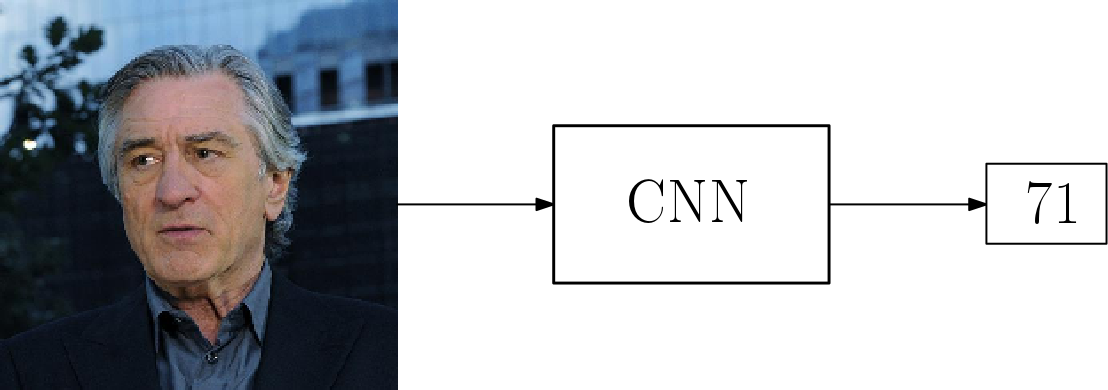
\includegraphics[width=\textwidth]{img/deniro_cnn}
     \label{fig:deniro_cnn}
\end{figure}

Os dados disponíveis para este contexto seráo particionados em três conjuntos disjuntos, sendo $70\%$ reservados para o treino, $10\%$ para validação e $20\%$ para teste. Esta partição obedece à tecnica \emph{Holdout} de validação cruzada.

Os modelos propostos para esta tarefa terão seu desempenho aferido perante os dados do conjunto de testes de acordo com a métrica de desempenho \emph{Root Mean Squared Error} (RMSE). Esta métrica observa a diferença entre cada um dos valores previstos $\hat{y}$ e os reais $y$, enquanto calcula uma média de uma maneira imune ao fato de os valores previstos poderem ser tanto maiores quanto menores que os valores reais. A Equação \ref{eq:rmse} representa o cálculo do RMSE \cite{brink2016real}.

\begin{equation}\label{eq:rmse}
     RMSE = \sqrt{\frac{1}{n} \sum_{i=1}^n (y_i - \hat{y})^2}
\end{equation}

\subsection{Conjunto de Dados}
%!TEX root = ../sbc-template.tex
Para a tarefa de aprendizado apresentada, dispôs-se da base de dados experimentais IMDb, composta de $452.132$ exemplares contendo imagens e outras informações de $20.284$ dos atores mais populares listados no site IMDb. O conjunto de dados foi construído utilizando técnicas de \emph{web crawling} aplicadas aos perfis de atores do site, em que foram coletadas todas as imagens relacionadas à celebridade, além de informações como data de nascimento, nome e gênero \cite{IMDb_derivada}.

A base de imagens oriunda do site IMDb foi organizada por Rothe et al. considerando uma tarefa de aprendizado análoga à deste trabalho, conforme mencionado na Seção  \ref{sec:trab_relac} \cite{rothe2015dex}.  Nesta base, há também as coordenadas da localização de um rosto detectado na imagem, além de uma pontuação atribuída ao rosto produzida pelo detector de face, quantificando o grau de certeza na detecção do rosto. Partindo da possibilidade de haver mais de um rosto por imagem, uma segunda pontuação é atribuída pelo detector, referente ao grau de certeza de que há outro rosto na mesma imagem.

Neste contexto, cada exemplo deste conjunto de dados é referente a uma imagem, cujos meta-dados estão descritos em seus atributos, que compreendem o nome, gênero, data de nascimento e um número de identificação da celebridade cujo perfil estava atrelado à imagem, o endereço da foto em disco, a suposta localização da face da celebridade, e pontuações referentes a duas possíveis faces encontradas. Assim, há exemplos de imagens em que há apenas um rosto, como mostrado na Figura \ref{tab:um_deniro}. Já na Figura \ref{tab:dois_deniro_correto} está o exemplo de uma imagem onde há mais de um rosto, porém a localização do rosto está correta. Por fim, na Figura \ref{tab:dois_deniro_errado} há uma imagem com mais de um rosto, porém o rosto identificado neste item não é o da celebridade cujos dados estão referenciados.

\begin{figure}[ht]
     \caption{Exemplo de imagem do conjunto de dados contendo apenas um rosto.}
     \label{tab:um_deniro}
          \begin{minipage}[c]{0.62\linewidth}
          \begin{small}
          \centering
          \begin{tabular}{p{3.3cm} p{5cm}}\toprule
               \textbf{Meta-dado} & \textbf{Valor} \\ \midrule
               ID Celebridade & 16349 \\
               Nome & Robert De Niro \\
               Endereço da imagem & \footnotesize{imdb$/$34$/$nm0000134$\_$rm334009 0368$\_$1943-8-17$\_$2011.jpg} \\
               Pontuação da Face & $5.21396$ \\
               Pontuação da Segunda Face & NaN \\
               Localização da Face & $(663.65, 992.475, $ $590.134, 918.959)$ \\
               Data de Nascimento  & $1943-08-17$\\
               Ano da Foto & 2011 \\
               Gênero & Masculino \\
               \bottomrule
          \end{tabular}
     \end{small}
     \end{minipage}
     \hfill
     \begin{minipage}[c]{0.35\linewidth}
          \centering
          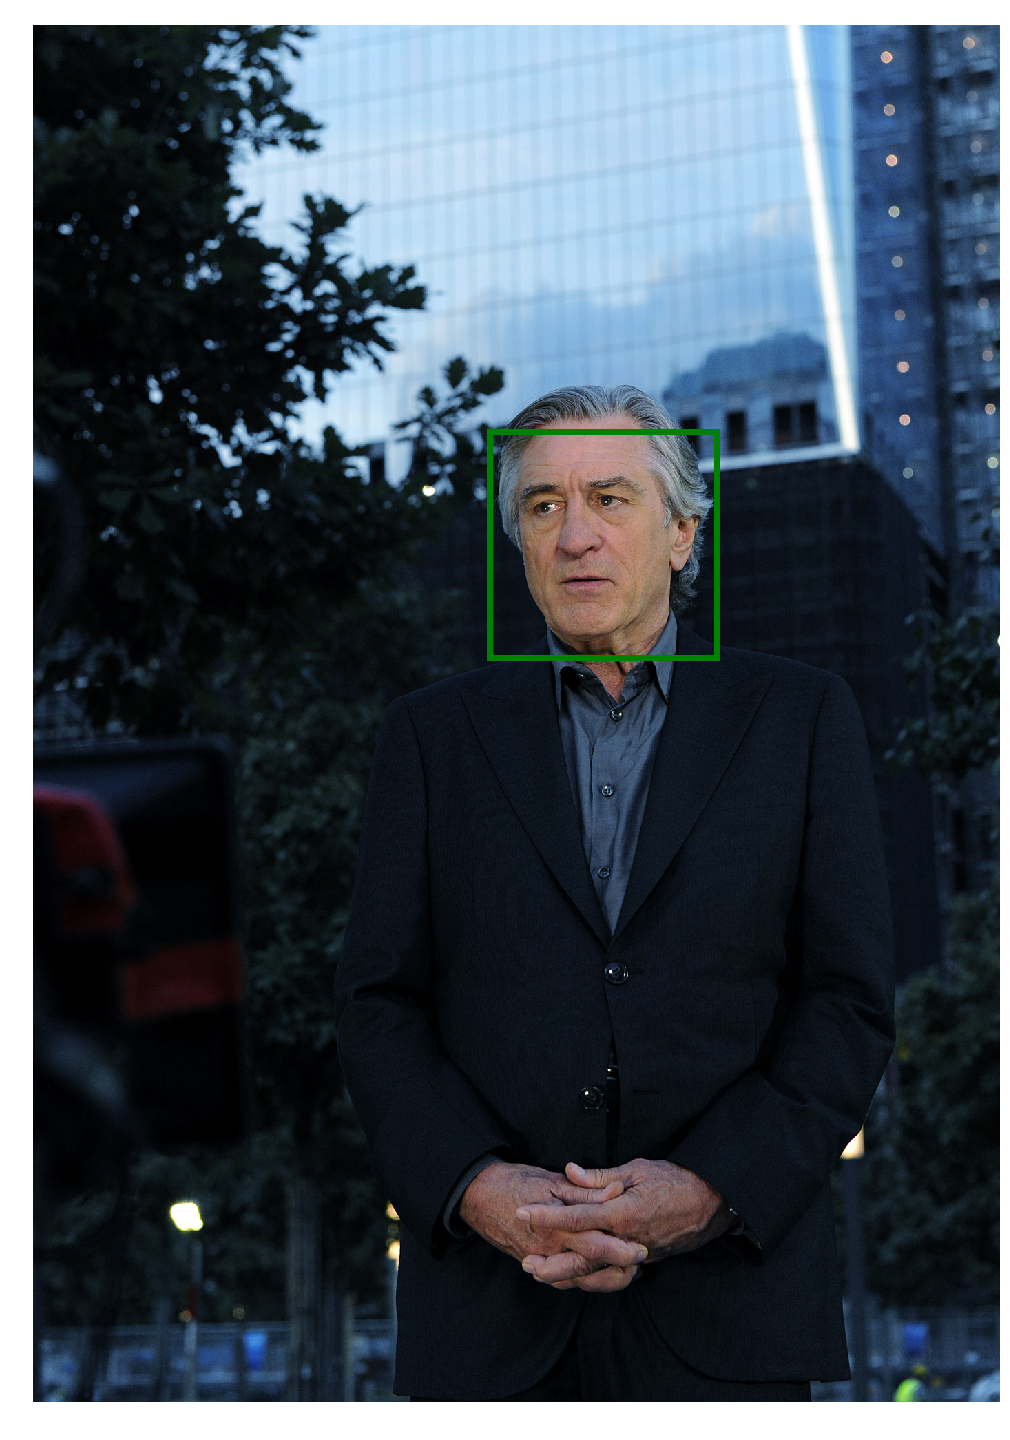
\includegraphics[width=\linewidth]{img/deniro_plt}
     \end{minipage}
\end{figure}

\begin{figure}[ht]
     \caption{Exemplo de imagem do conjunto de dados contendo mais de um rosto com a classificação correta.}
     \label{tab:dois_deniro_correto}
          \begin{minipage}[c]{0.62\linewidth}
          \begin{small}
          \centering
          \begin{tabular}{p{3.3cm} p{5cm}}\toprule
			   \textbf{Meta-dado} & \textbf{Valor} \\ \midrule
               ID Celebridade & 16349 \\
               Nome & Robert De Niro \\
               Endereço da imagem & \footnotesize{imdb$/$34$/$nm0000134$\_$rm17663 60064$\_$1943-8-17$\_$2010.jpg} \\
               Pontuação da Face & $5.12527$ \\
               Pontuação da Segunda Face & $5.08887$ \\
               Localização da Face & $(914.886, 1426.31, $ $287.31, 798.734)$ \\
               Data de Nascimento  & $1943-08-17$\\
               Ano da Foto & 2010 \\
               Gênero & Masculino \\
               \bottomrule
          \end{tabular}
     \end{small}
     \end{minipage}
     \hfill
     \begin{minipage}[c]{0.35\linewidth}
          \centering
          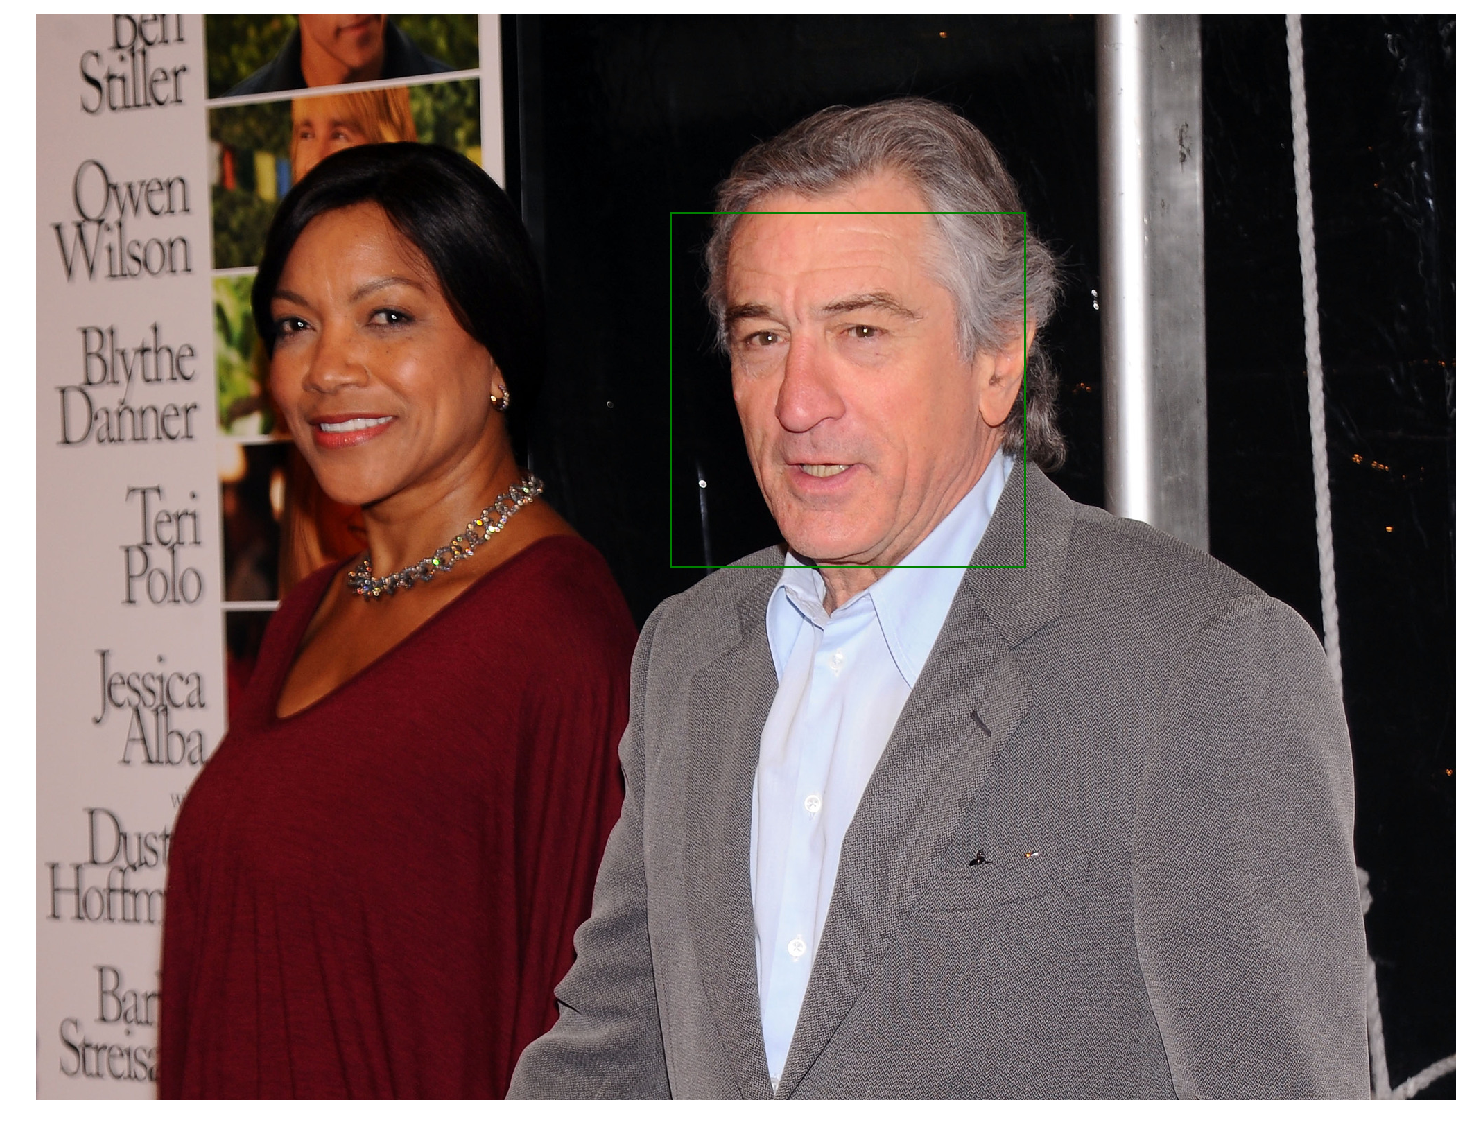
\includegraphics[width=\linewidth]{img/deniro_many_plt_correto}
     \end{minipage}
\end{figure}

\begin{figure}[ht]
     \caption{Exemplo de imagem do conjunto de dados contendo mais de um rosto com a classificação errônea.}
     \label{tab:dois_deniro_errado}
          \begin{minipage}[c]{0.62\linewidth}
          \begin{small}
          \centering
          \begin{tabular}{p{3.3cm} p{5cm}}\toprule
               \textbf{Meta-dado} & \textbf{Valor} \\ \midrule
               ID Celebridade & 16349 \\
               Nome & Robert De Niro \\
               Endereço da imagem & \footnotesize{imdb$/$34$/$nm0000134$\_$rm14800 44288$\_$1943-8-17$\_$2012.jpg} \\
               Pontuação da Face & $5.51656$ \\
               Pontuação da Segunda Face & $4.55379$ \\
               Localização da Face & $(1392.72, 1614.18, $ $225.55, 447.003)$ \\
               Data de Nascimento  & $1943-08-17$\\
               Ano da Foto & 2012 \\
               Gênero & Masculino \\ \bottomrule
          \end{tabular}
     \end{small}
     \end{minipage}
     \hfill
     \begin{minipage}[c]{0.35\linewidth}
          \centering
          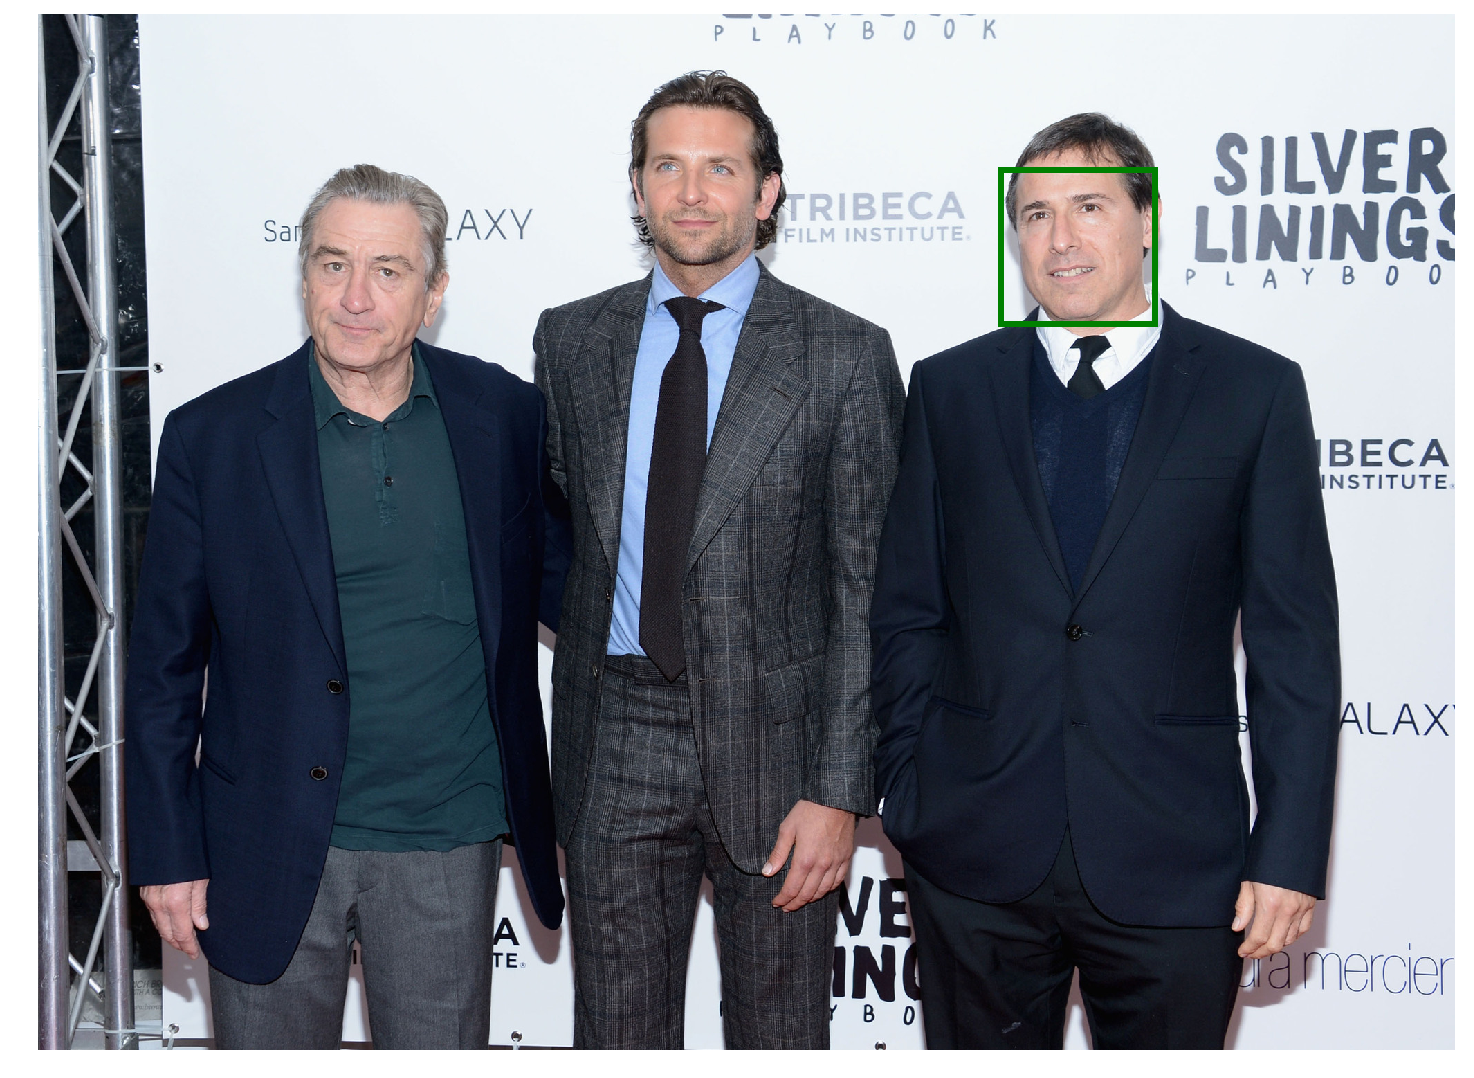
\includegraphics[width=\linewidth]{img/deniro_many_plt_errado}
     \end{minipage}
\end{figure}

A versão original das imagens do conjunto de dados IMDb ocupava 267 GB em disco. Porém, uma versão pré-processada dessas imagens está disponível, contendo as faces recortadas com $40\%$ da largura e altura da imagem original, totalizando $7,1$ GB de dados. Esta versão foi considerada neste trabalho.


\subsection{Limpeza e Pré-processamento dos dados}

A fim de adequar melhor o conjunto de dados para os modelos de CNNs utilizados, realizou-se uma limpeza e pré-processamento dos meta-dados e das imagens da base IMDb, que se iniciou com o cálculo do atributo alvo, a idade, a partir dos atributos originais fornecidos. A idade foi aferida através da data de nascimento da celebridade e do ano em que a fotografia em questão foi capturada. A data de nascimento estava no formato \emph{datenum}, sendo necessária a conversão desta medida para a data comum, de onde foi extraído o ano de nascimento. A seguir, calculou-se a idade a partir da diferença entre o ano de nascimento da celebridade e o ano em que a foto foi tirada.

Uma análise do conjunto de dados revelou a presença de itens com idade e gênero apresentando valores nulos, inválidos ou negativos, que foram descartados. Observou-se também a presença de múltiplos exemplos referentes à mesma pessoa com a mesma idade. Houve a remoção de tais exemplos, a fim de evitar que a apresentação de um mesmo rosto com a mesma idade \emph{overfitting} nos modelos. Exemplos atípicos, possivelmente resultado de rotulação incorreta, como idade maior que $100$ anos ou não compatível com os dados da celebridade referida nos meta-dados também foram descartados \todo{mostrar exemplo}. Os atributos de pontuação de rostos foram úteis para identificar e remover exemplos em que não havia nenhum rosto identificado, ou em que havia mais de uma face na imagem. Este descarte foi realizado com o objetivo de eliminar rotulações errôneas, como a mostrada na Tabela \ref{tab:deniro_many_plt_errado}.

A última etapa consistiu na padronização das dimensões da imagem. Considerando a literatura, definiu-se o tamanho para $224 \times 224$ e o modo RGB como padrões. Por fim, após a padronização das imagens de entrada, o cálculo do atributo alvo idade, a adequação do caminho para as imagens em disco e a remoção de exemplos impróprios, seguiu-se o descarte dos outros meta-dados irrelevantes para a tarefa de estimação de idade de um indivíduo a partir de imagem. A data em que a foto foi tirada, o nome, número de identificação, gênero, data de nascimento, localização do rosto da celebridade e pontuações de rostos nas imagens foram removidos.

Por fim, o conjunto de dados utilizado consiste de $47950$ exemplos contendo imagens e idades disjuntas de $14607$ celebridades. O histograma de frequência de idades de 0 a 100 anos pode ser visualizado na Figura \ref{fig:hist}. Este total foi dividido em conjunto de treinamento, contendo $70\%$ da base, ou $33565$ exemplos; conjunto de validação, referente a $10\%$ dos dados, ou $4795$ itens; e conjunto de testes, contendo os restantes $20\%$, ou $9590$ exemplos.

\begin{figure}
     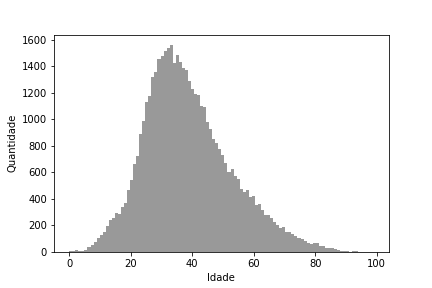
\includegraphics[width=0.7\textwidth]{img/idade_hist_clean}
     \caption{Histograma de frequência da idade do conjunto de dados utilizado.}
     \label{fig:hist}
\end{figure}

\subsection{Modelos de CNN Considerados}
Considerou-se as arquiteturas LeNet e AlexNet. Todas as funções de ativação tangente hiperbólica foram substituídas pela ReLU. A implemetação da AlexNet seguiu a prática atual de utilizar apenas uma GPU no treinamento, portanto as camadas dividas foram unificadas. A normalização original que utilizava LBN foi substituída pela normalização em batch, que tem se mostrado mais efetiva \todo{citar chollet}.

\subsection{Parâmetros e Hiperparâmetros}

\subsection{Métricas de Desempenho}

% Escrever sobre micro-averaging
% \subsubsection{Micro-Média}
% \todo{como traduzir?}
% A micro-média é uma medida de performance utilizada em problemas de classificação multi-classe em que não há balanceamento entre os elementos de cada tipo. Assim, cada classe recebe um peso de acordo com sua frequência entre os exemplos, o que faz com que o $F1$-score das classes com mais exemplos infuencie na métrica mais que o de classes com menos exemplos \cite{ghamrawi2005collective}. A performance é dada pela média de todos os exemplos como se pertencessem a uma mesma classe, como mostra a Equação \ref{eq:micro_averaging}, sendo $PR$, $Re$ e $F1$ a precisão, revocação e $F1$-score, respectivamente, e TP, FP, FN, positivo verdadeiro, positivo falso e negativo verdadeiro\cite{kubat2016introduction}.
% \begin{align}\label{eq:micro_averaging}
% 	\begin{split}
% 		Pr^{\mu} = \frac{\sum_{i=1}^L TP_i}{\sum_{i=1}^L TP_i + FP_i}
% 		\\ \\
% 		Re^{\mu} = \frac{\sum_{i=1}^L TP_i}{\sum_{i=1}^L TP_i + FN_i}
% 		\\ \\
% 		F1^{\mu} = \frac{2 \times Pr^{\mu} \times Re^{\mu}}{Pr^{\mu} + Re^{\mu}}
% 	\end{split}
% \end{align}

\subsection{Etapa de Treinamento}

\subsection{Etapa de Testes}
